% TODO: replace this image with our own renders
\begin{figure}[H]
	\centering
	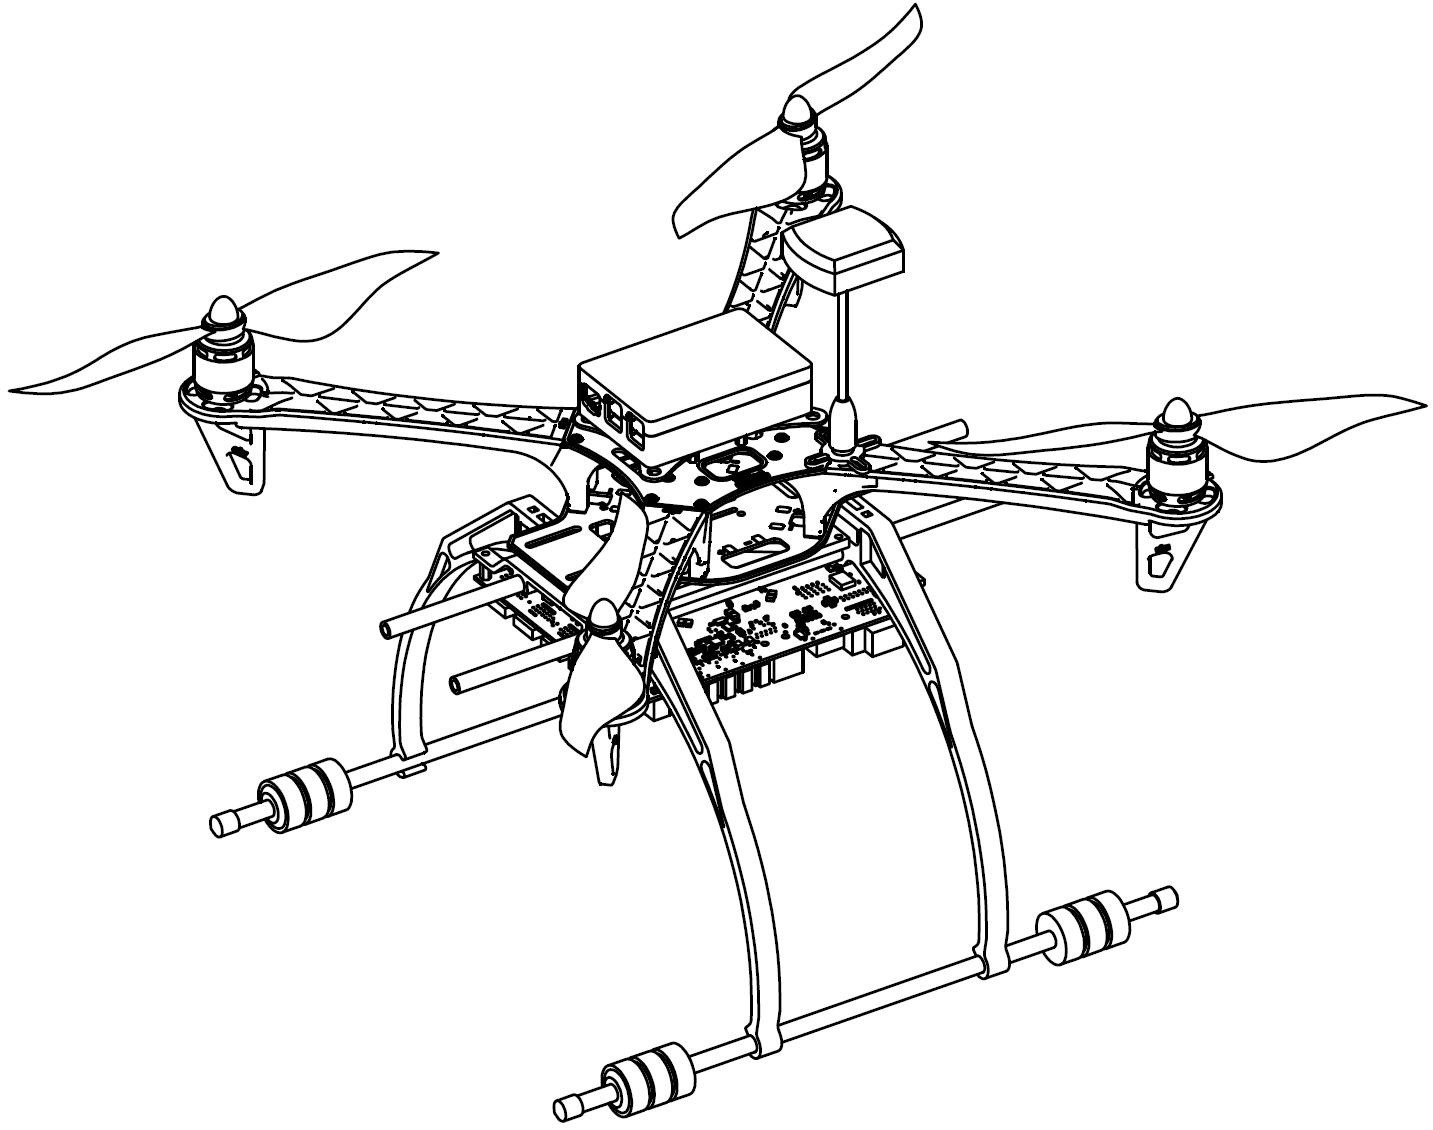
\includegraphics[width=0.85\textwidth]{img/testrigcad1.png}
	\caption[Team 109 Testing Rig Prototype]{Team 109 Testing Rig Prototype using RPAS Generously Provided by Yiyi Yan and UBC \textit{Unmanned Aerial Systems}}
	\label{fig:testrigcad1}
\end{figure}

A remote-piloted aerial system (RPAS) or sometimes referred to as ``drone" and ``multirotor" consists of serveral subsystems: airframe, mechanical structures, propulsion, battery, sensors, and flight computer. This section will explore these subsystems in more detail. Figure~\ref{fig:testrigcad1} is a render of the completed mutlirotor with the computing platform payload attached.

\subsubsection{Mechanical}
The mechanical subsystem of the multirotor is comprised of the frame that holds all the propulsion system, on-board computer and sensors, and the payload together.

\paragraph{Frame Configuration}

\begin{figure}[b]
	\centering
	\begin{subfigure}[b]{0.3\textwidth}
		\centering
		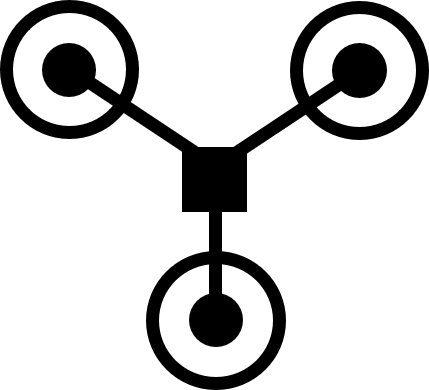
\includegraphics[scale=0.4]{img/drone_yconfig}
		\caption{Tricopter Y-Configuration}
		\label{fig:tricopter-y}
	\end{subfigure}
	~
	\begin{subfigure}[b]{0.3\textwidth}
		\centering
		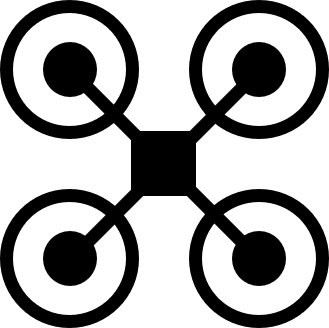
\includegraphics[scale=0.4]{img/drone_xconfig}
		\caption{Quadcopter X-Configuration}
		\label{fig:quadcopter-x}
	\end{subfigure}
	~
	\begin{subfigure}[b]{0.3\textwidth}
		\centering
		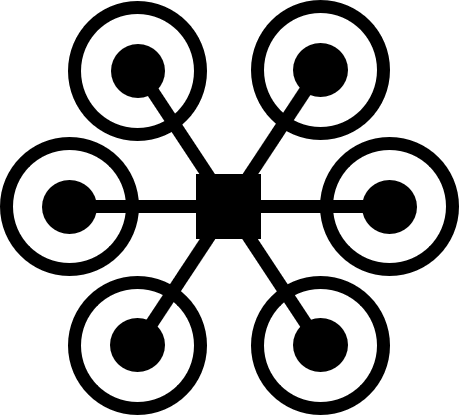
\includegraphics[scale=0.4]{img/drone_hexconfig}
		\caption{Hexcopter X-Configuration}
		\label{fig:hexcopter-x}
	\end{subfigure}
	
	\caption{Multirotor RPAS Configurations}
	\label{fig:rpas-config}
\end{figure}

\begin{figure}[h]
	\centering
	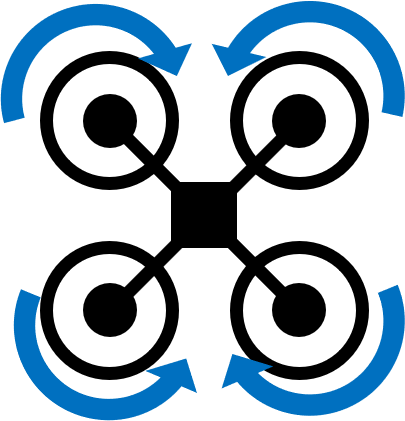
\includegraphics[scale=0.4]{img/drone_xconfigt}
	\caption{Quadcopter X-configuration}
	\label{fig:quadcopter-x-t}
\end{figure}

\begin{figure}[h]
	\centering
	\begin{subfigure}[b]{0.3\textwidth}
		\centering
		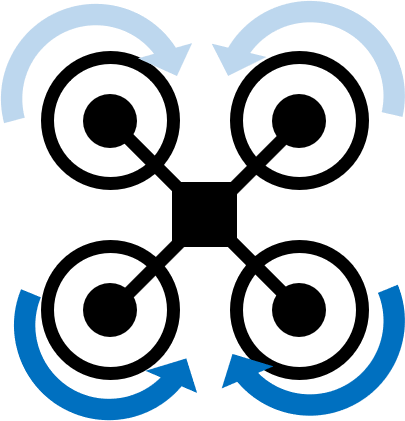
\includegraphics[scale=0.4]{img/drone_x_pitch}
		\caption{Pitch forward}
		\label{fig:x-pitch}
	\end{subfigure}
	~
	\begin{subfigure}[b]{0.3\textwidth}
		\centering
		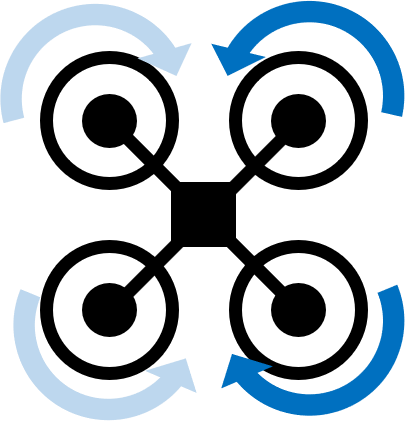
\includegraphics[scale=0.4]{img/drone_x_roll}
		\caption{Roll left}
		\label{fig:x-roll}
	\end{subfigure}
	~
	\begin{subfigure}[b]{0.3\textwidth}
		\centering
		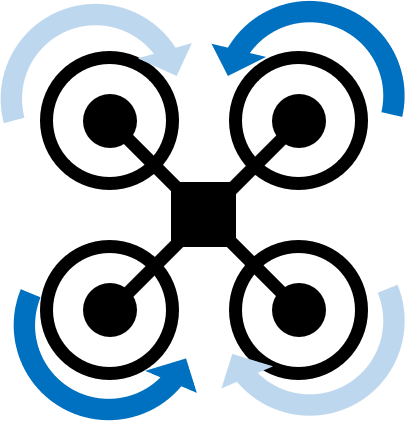
\includegraphics[scale=0.4]{img/drone_x_yaw}
		\caption{Yaw left}
		\label{fig:x-yaw}
	\end{subfigure}
	
	\caption{Using differential thrust to obtain 6-DOF movement. }
	\label{fig:rpas_6dof}
\end{figure}

A multirotor has several common configurations such as tricopter, quadcopter, hexacopter as depicted in Figure~\ref{fig:rpas-config}. Because each frame has different layouts of motors, the forces acting on the drone is inherently different and thus provides advantages and disadvantages of their own.

We use a quadcopter X4 configuration (4 motors and propellers in the shape of a letter X) for our multirotor as it is easy to control and provides abundant control system robustness. Such configuration is also the most popular amongst the UAS industry because it is balances redundancy and robustness with capacity and performance.

As seen in Figure \ref{fig:quadcopter-x-t}. Two of the motors spin clockwise and the other two spin counter-clockwise --- effectively canceling each other's unintended torque applied to the multirotor. Applying the same power into each motor allows the MRPAS to hover in place. We can perform 6 degree-of-freedom (DOF) movements by applying a combination of differential thrusts to each motor (Figure \ref{fig:rpas_6dof}). An X4 configuration is inherently stable.

A dual-blade helicopter, for example, requires fewest number of motors. But like a single-blade helicopter, the system in control theory sense, is naturally unstable and requires difficulty to stabilize the system. A tricopter has odd number of motors which also shares similar characteristics with a helicopter where the system requires an additional tail motor to compensate for the uneven torque. 

Configurations using more than 4 motors such as a hexacopter or an octocopter are very expensive for the amount of parts they require. Drones of these configuration classes are very stable with failure redundancy. However, these drones are typically much larger (0.6m to 1.5m wide) and much heavier (up to 25 kg). As a result, they are typically used in industrial, filming, and agriculture applications with a typical unit cost of at least several thousand dollars. These configurations are not suitable for our applications.

\paragraph{Airframe}

\begin{figure}[h]
	\centering
	\begin{subfigure}[b]{0.33\textwidth}
		\centering
		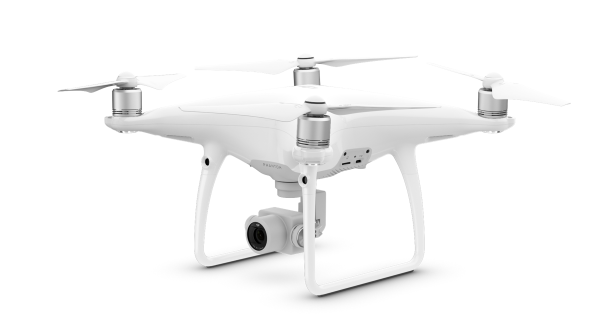
\includegraphics[width=\textwidth]{img/djiphantom4}
		\caption{DJI Phantom 4 (350 mm)}
		\label{fig:djiphantom}
	\end{subfigure}
	~
	\begin{subfigure}[b]{0.33\textwidth}
		\centering
		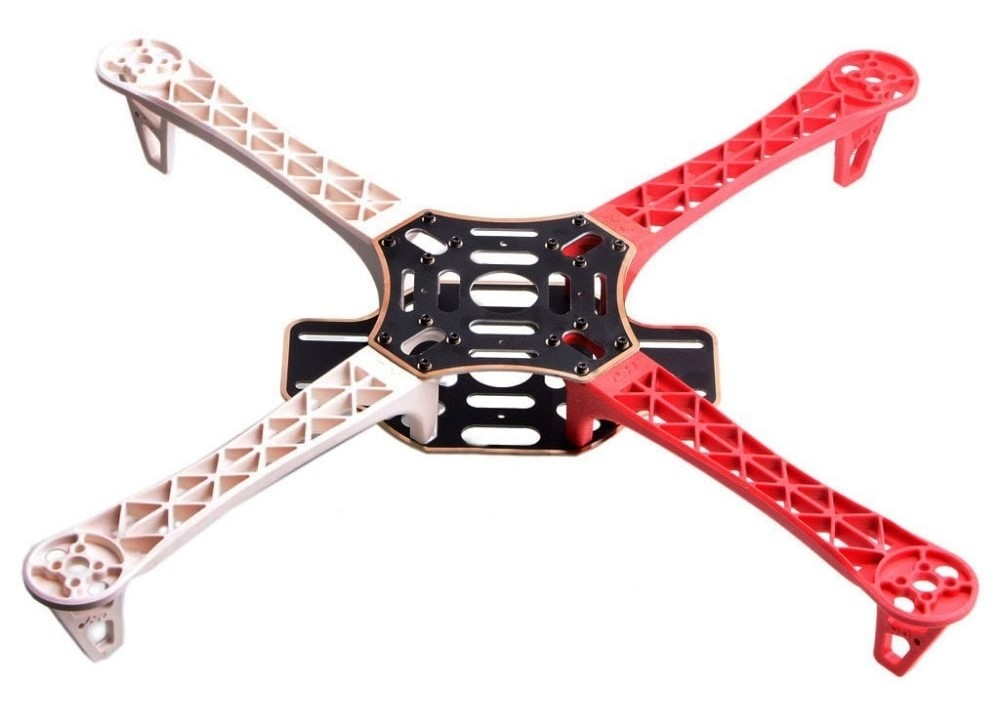
\includegraphics[width=\textwidth]{img/f450frame}
		\caption{Generic DIY frame kit (450 mm)}
	\end{subfigure}
	~
	\begin{subfigure}[b]{0.33\textwidth}
		\centering
		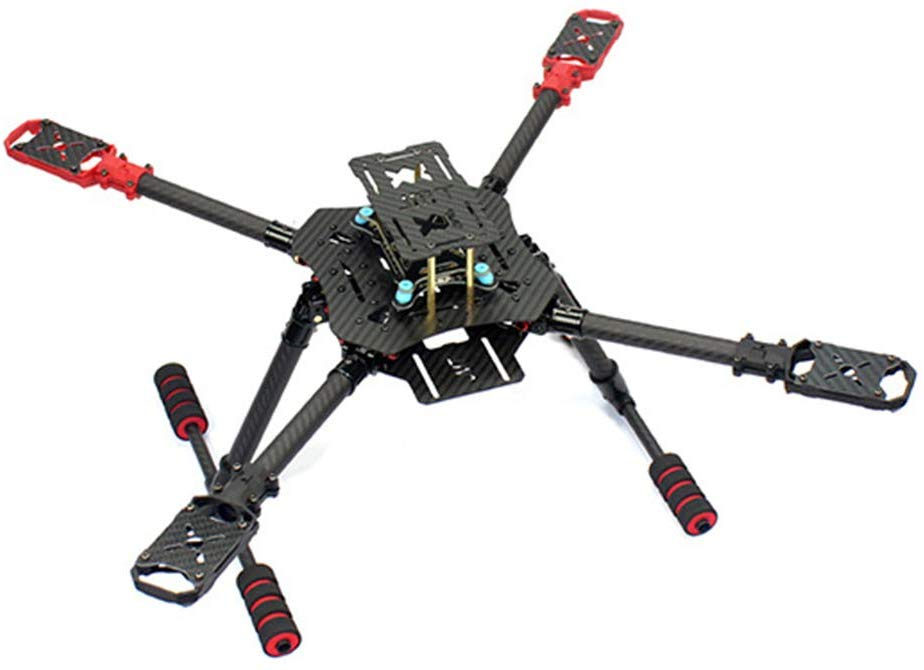
\includegraphics[width=\textwidth]{img/jmt560}
		\caption{JMT X4 Carbon Fiber Frame (560 mm)}
		\label{fig:jmtx4}
	\end{subfigure}
	~
	\begin{subfigure}[b]{0.33\textwidth}
		\centering
		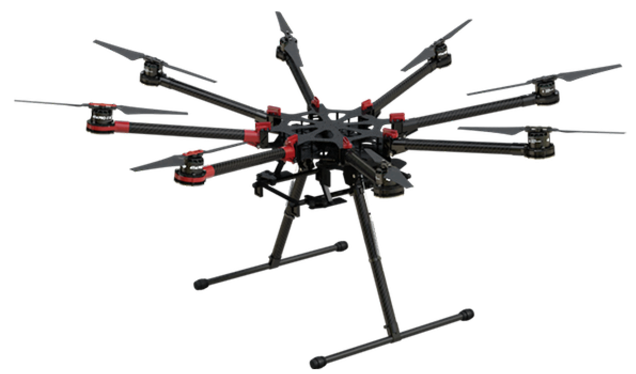
\includegraphics[width=\textwidth]{img/djis1000}
		\caption{DJI Spreadwings S1000 (1000 mm)}
		\label{fig:djis1000}
	\end{subfigure}
	
	\caption{Air Frame Options with Various Size Tiers }
\end{figure}

Multirotor airframe sizes are commonly designated by their \textit{motor-to-motor-diagonal-span} (MMDS), which measures the distance between the pair of motors which are the furthest apart. 

We adopt a X4 560 mm MMDS carbon fibre frame from JMT, as shown in Figure~\ref{fig:jmtx4}. The frame is carbon fibre to enhance structural rigidity while keeping the system relatively lightweight. The frame features foldable arms and landing gears for portability, but we consider replacing the hinges with static parts to reduce  weight and achieve a longer flight time. The X4 560 mm frame is also wide enough to support propellers up to 14 inches in diameter. 

The 350 mm frames are also popular amongst consumer products such as the DJI Phantom series\cite{dji-phantom-3-specs} as seen in Figure~\ref{fig:djiphantom}. A frame size of 350 mm would constrain our ability to mount larger hardware --- posing a significant risk to integrating computing platform hardware. Additionally, the 350 mm size also limits the propeller maximum size. The largest quadcopter configurations have an MMDS of 1000 mm to allow for extremely large payload capacities such as the one shown in Figure~\ref{fig:djis1000}. However, these are more commonly used for industrial or military applications.

\paragraph{Customized Add-ons}
% TODO: add CAD parts

\subsubsection{Propulsion}


\paragraph{Motor Type}
\paragraph{Electronic Speed Controllers}
\paragraph{Propellers}

\subsubsection{Battery and Electrical Systems}
\paragraph{Battery Type}
\paragraph{Battery Capacity}
\paragraph{Power Distribution}

\subsubsection{Flight Computer and Sensors}
\paragraph{Flight Computer Unit}
\paragraph{Sensors}
\paragraph{Flight Modes}
\paragraph{FCU Software}

\subsubsection{Communication and Control}
\paragraph{Transmitter}
\paragraph{Receiver}